\documentclass[pdf]
{beamer}
\mode<presentation>{}

\usepackage{amsmath}

\newcommand\bayeseq{\mathrel{\overset{\makebox[0pt]{\mbox{\normalfont\tiny\sffamily Bayes}}}{=}}}

%% preamble
\title{Model inference from protein time-course in Hematopoietic Stem Cells (HSC)}
\subtitle{}
\author[shortname]{Pandu Raharja \inst{1, 2} \and Rene Schoeffel \inst{1, 2} \and Michael Strasser \inst{3}}
\institute[shortinst]{\inst{1} Technische Universit\"at M\"unchen \and %
                      \inst{2} Ludwig-Maximilians-Universit\"at M\"unchen \and %
                      \inst{2} Institute of Computational Biology (ICB), Helmholtz Zentrum M\"unchen}
\begin{document}

%% title frame
\begin{frame}
\titlepage
\end{frame}

%% normal frame
\begin{frame}{Introduction}
	\begin{itemize}
		\item Dynamics of hematopoetic stem cell maturation cell from Common Myeloid Progenitor (CMP) to Megakaryocyte-Erythroid Progenitor (MEP) and Granulocyte-Macrophage Progenitor (GMP)
	\end{itemize}
	
	\begin{figure}[ht]
		\begin{center}
			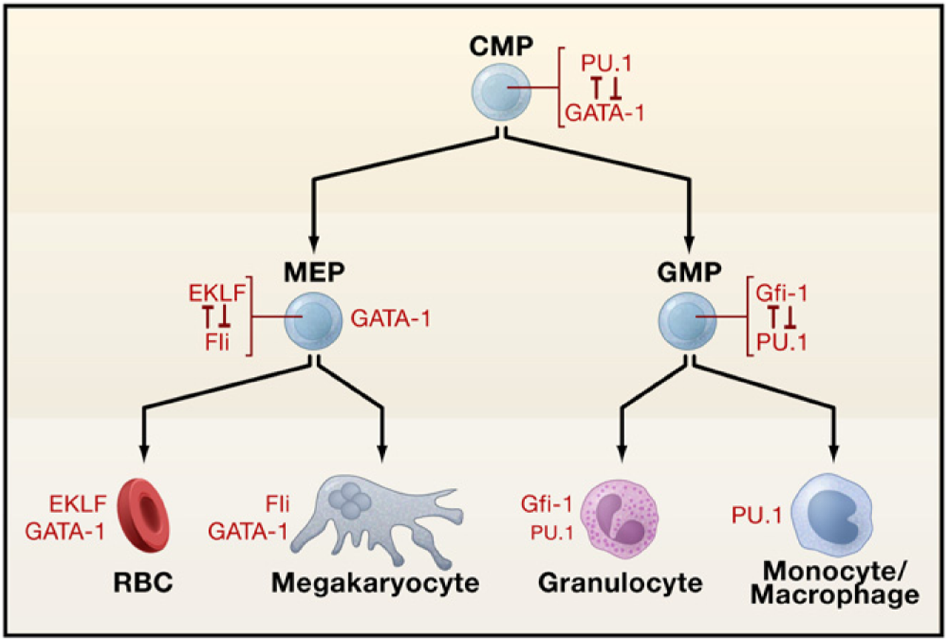
\includegraphics[height=2in]{figures/homatopoietic_focus.png}
			~\footnote{Graf \& Enver, 2009, \textit{Nature}}
		\end{center}
	\end{figure}
\end{frame}

\begin{frame}{Introduction (cont'd)}
	\begin{itemize}
		\item Assumed corss-inhibition dynamics between \texttt{Pu.1} and \texttt{Gata1} in cell maturation fate:
	\begin{itemize}
		\item Dynamics is assumed to be a bistable toggle-switch system
		\item Lineage decision is a stochastics process resulting in uneven yield of MEP and GMP (70\% : 30\%)
	\end{itemize}
	\item Analysis on single-cell time-lapsed data to infer parameters of this dynamics
	\end{itemize}
	\begin{figure}[ht]
		\begin{center}
			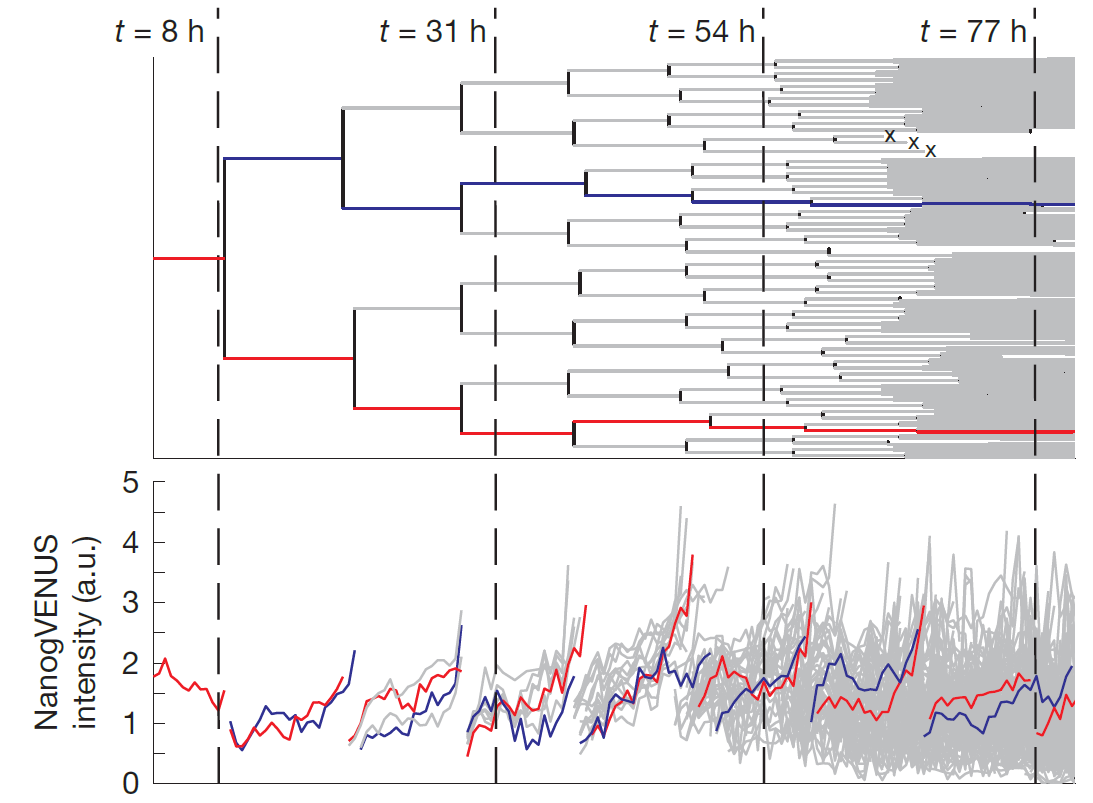
\includegraphics[height=1.5in]{figures/cell-generations.png}
			~\footnote{Feigelman, 2016, Ph.D. Thesis}
		\end{center}
	\end{figure}
\end{frame}

\begin{frame}{Problems}
	\begin{itemize}
	\item Stochaticity in single cell resolution is more punctuated
	\item Tree structure of the data add ore complexity: inheritance of information during inference process is not trivial
	\end{itemize}
\end{frame}

\begin{frame}{Ideas}
	\begin{itemize}
	\item Sequential Monte Carlo simulations along the time-apsed data to infer "good" parameters
	\item<2-> \textbf{problem:} Overfitting due to single-cell biased
	\item<3-> \textbf{solution:} Inference across cell lineages
	\item<4-> Inferred parameters from all simulated lineages are represented as distribution
	\item<5-> Final inferred parameters are expected value $E$ of the distribution
	\end{itemize}
\end{frame}

\begin{frame}{Particle Filtering}

	\begin{itemize}

	\item \textbf{Particle}
	A particle K is defined as a triple of previous simulation trajectory $X$, parameter set $\theta$ and
assumed model $M$,

		\begin{equation}
		K := (X, \theta, M)
		\end{equation}
		
	\item \textbf{Particle filtering} is an parameters inference method that consists of: (1) \textit{sequentially} performing simulations using \textit{particles}, (2) \textit{updating} the \textit{prior} assumptions of the model using the results of the simulations and (3) rerunning the simulations using updated assumptions (\textit{posterior}).
	
	\end{itemize}

\end{frame}

\begin{frame}{Particle Filtering: update rule}

	\begin{itemize}
	\item \textbf{Posterior}
	
	After each simulation step, a posterior describes the probability of having the trajectory $X$ and
parameter $\theta$ given the observation $D$ from real data,

	\begin{equation}
	P (X, \theta |D) \bayeseq \frac{P(D|X, \theta) P(X, \theta)}{P(D)}
	\end{equation}
	
	This Bayesian update rule is used to update parameters by looking at how well does the simulation follow the real data. I.e. after an iteration we will choose parameters belonging to particles that simulate the trajectory well w.r.t. experimental data.
	
	\item \textbf{Gamma Distribution} is used as prior since a posterior of a gamma is in turn gamma distributed (\textit{prior conjugate}).
	\end{itemize}
	
\end{frame}

\begin{frame}{Particle Filtering: algorithm}
	\begin{enumerate}
		\item Initialization of parameters $\theta$.
		\item Input of data $\mathcal{D}$.
		\item Particle filtering routine:

		\begin{enumerate}
			\item Generation of initial particles for step i
			
			\begin{equation}
				Ki := (K_{i1}, K_{i2}, \dots, K_{im})
			\end{equation}

			\item Simulation run of each particle $K_{ij}$
			\item Weighting of each particle. The weight is a function of the probability of observing the data given the simulation result.

			\begin{equation}
				w_i^k = P(D_i | X_i^k) = \mathcal{N}(\mathcal{D}_i | X_i^k)
			\end{equation}

			\item Parameter update for every K,

			\begin{equation}
				\theta^k \propto P(\theta | X^k_{[to, ti]})
			\end{equation}

		\end{enumerate}

	\end{enumerate}
\end{frame}

\begin{frame}{Particle Filtering: visualization}
	\begin{figure}[ht]
		\begin{center}
			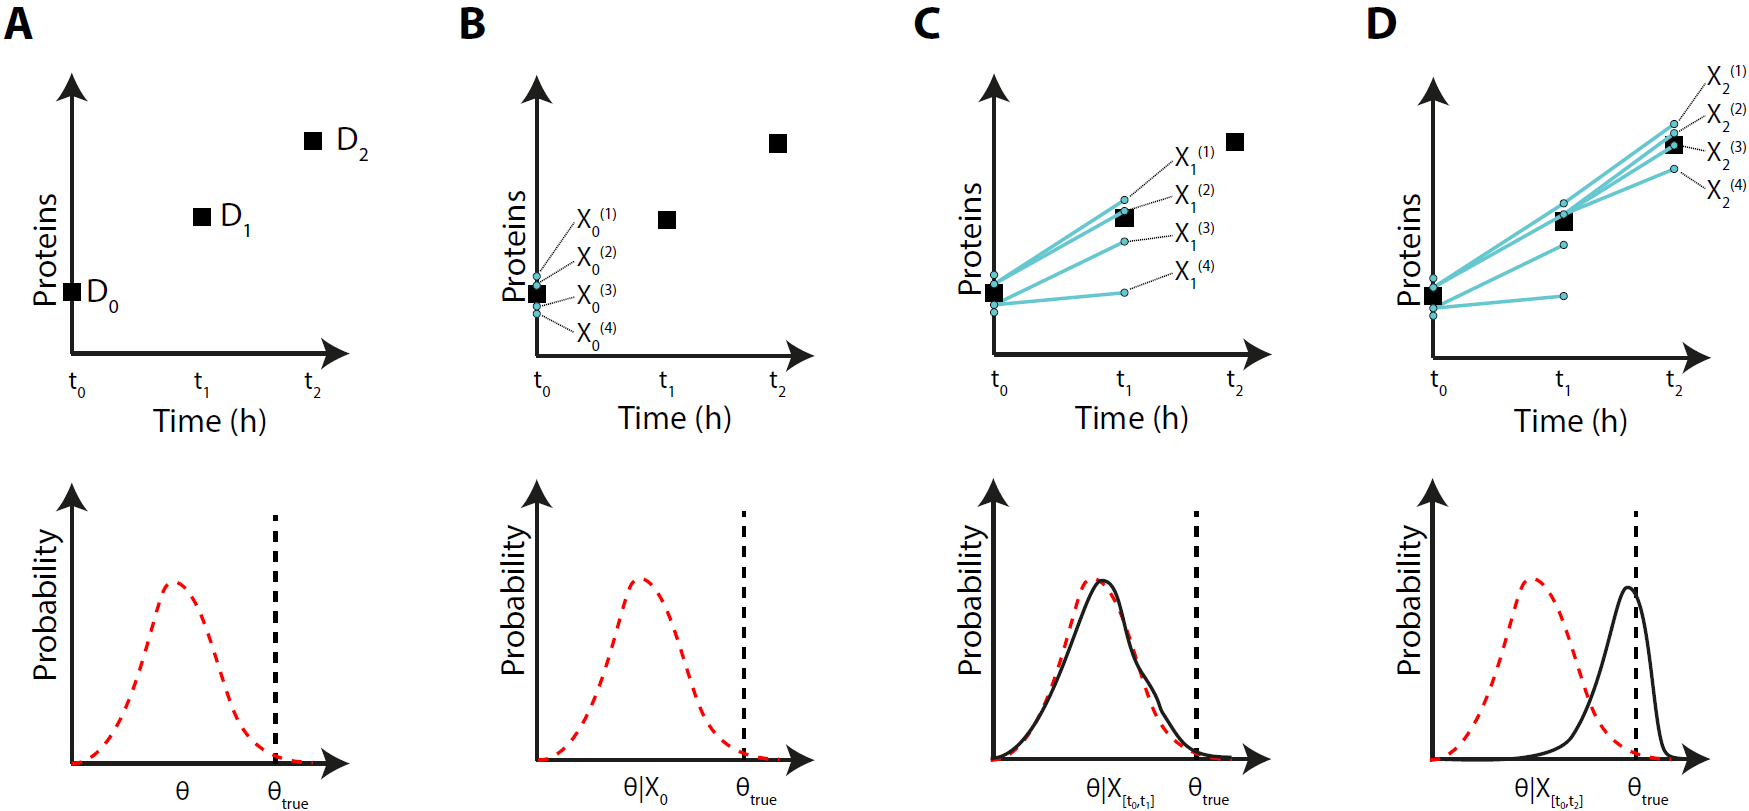
\includegraphics[height=2in]{figures/particle_filtering.png}
			~\footnote{Feigelman, 2016, Ph.D. Thesis}
		\end{center}
	\end{figure}
\end{frame}

\end{document}